%!TEX TS-program = xelatex
\documentclass[]{friggeri-cv}
\usepackage{afterpage}
\usepackage{hyperref}
\usepackage{color}
\usepackage{xcolor}
\usepackage{smartdiagram}
\usepackage{fontspec}
% if you want to add fontawesome package
% you need to compile the tex file with LuaLaTeX
% References:
%   http://texdoc.net/texmf-dist/doc/latex/fontawesome/fontawesome.pdf
%   https://www.ctan.org/tex-archive/fonts/fontawesome?lang=en
%\usepackage{fontawesome}
%\oddsidemargin=-1cm
\textwidth=15cm
%\marginparwidth = -3cm
\textheight=26cm

\usepackage{metalogo}
\usepackage{dtklogos}
\usepackage[utf8]{inputenc}
\usepackage{tikz}
\usetikzlibrary{mindmap,shadows}
\hypersetup{
    pdftitle={},
    pdfauthor={},
    pdfsubject={},
    pdfkeywords={},
    colorlinks=false,           % no lik border color
    allbordercolors=white       % white border color for all
}
\smartdiagramset{
    bubble center node font = \footnotesize,
    bubble node font = \footnotesize,
    % specifies the minimum size of the bubble center node
    bubble center node size = 0.5cm,
    %  specifies the minimum size of the bubbles
    bubble node size = 0.5cm,
    % specifies which is the distance among the bubble center node and the other bubbles
    distance center/other bubbles = 0.3cm,
    % sets the distance from the text to the border of the bubble center node
    distance text center bubble = 0.5cm,
    % set center bubble color
    bubble center node color = pblue,
    % define the list of colors usable in the diagram
    set color list = {lightgray, materialcyan, orange, green, materialorange, materialteal, materialamber, materialindigo, materialgreen, materiallime},
    % sets the opacity at which the bubbles are shown
    bubble fill opacity = 0.6,
    % sets the opacity at which the bubble text is shown
    bubble text opacity = 0.5,
}

\addbibresource{bibliography.bib}
\RequirePackage{xcolor}
\definecolor{pblue}{HTML}{182333}
\definecolor{pblue2}{HTML}{d7edf5}
\definecolor{porange}{HTML}{e9511d}

\begin{document}
\smartdiagramset{border color = pblue,
    set color list={pblue!70,pblue2,porange,pblue2!90,pblue!80, pblue2, porange}, 
    bubble center node color = porange}
\header
      	{\hspace{15cm}\raisebox{-3ex}{
\includegraphics[scale=0.06]{img/Logo_Color_HorizontalEN.png}}
}
	{\raisebox{-2ex}{\begin{minipage}{\textwidth \normalsize}
		\begin{tabular}{r}
		Areas of interest:\\
		\begin{tabular}{l r}
					\textbf{DATA SCIENCE}&\textbf{FINANCES}\\
					\textbf{MACHINE LEARNING}&\textbf{\hspace{0.3cm}SAMPLING}
		\end{tabular}
	\end{tabular}
\end{minipage}}
}{}

% Fake text to add separator      
\vspace{-0.3cm}
\fcolorbox{white}{pblue2}{\parbox{\dimexpr\textwidth-2\fboxsep-2\fboxrule}{%
$\qquad$
}}

% In the aside, each new line forces a line break
\begin{aside}
  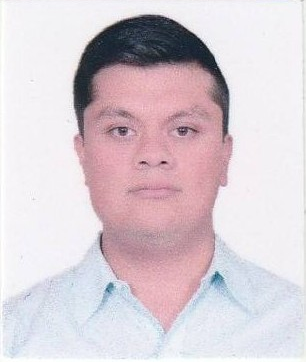
\includegraphics[scale=0.268]{img/foto2.png}
  \section{Phone}
    +521 5531560997
  \section{Mail}
    \href{mailto:victorm.garcia@comunidad.unam.mx}{\textbf{victorm.garcia@}\\comunidad.unam.mx}
    \href{mailto:victor.garcia@cimat.mx}{\textbf{victor.garcia@}\\cimat.mx}
    \section{Linkedin}
    \url{linkedin.com/in/victorm-garcia}%{linkedin.com/in/víctorm-garcia}
    \section{Portfolio}
    \url{victorgarciads.github.io}%{victorgarciads.github.io/}
     \section{Additional languages}
    \textbf{C1 level English}
  % use  \hspace{} or \vspace{} to change bubble size, if needed
  \section{Software}
\smartdiagram[bubble diagram]{
       \textbf{\vspace{1mm}R},
       \textbf{\vspace{1mm}LaTeX},
       \textbf{C/C++},
        \textbf{\vspace{1mm}Python},
        \textbf{\vspace{1mm}Git},
        \textbf{\vspace{1mm}Office},
        \textbf{\vspace{1mm}Hadoop/}\\\textbf{\vspace{1mm}Spark},
        \textbf{\vspace{-2mm}SQL}
    }\vspace{0.5cm}
  \section{Competencies \& Skills}
    \smartdiagram[bubble diagram]{
       \textbf{\vspace{2mm}Resilience},
	\textbf{Critical}\\\textbf{thinking},
	 \textbf{Complex}\\\textbf{problem}\\\textbf{solving},
	\textbf{Emotional}\\\textbf{intelligence},
        \textbf{Interpersonal}\\\textbf{skills},
    }
    ~
\end{aside}
\textbf{Professional Summary:}
Data scientist with research experience in interdisciplinary projects with interest in joining the data analysis area. Disciplined, fast learner and easily adaptable. With a willingness to work in a team and the ability to meet objectives with predefined times. Results-oriented.
\vspace{-0.4cm}
\section{Professional experience}
\vspace{-0.4cm}
\begin{entrylist}
\entry
   {   \begin{tabular}{r}
    		\hspace{0.85cm}03/20-today\\
     		
\includegraphics[scale=0.04]{img/Logo_Solo_Figura_Color.png}
	\end{tabular}
    }
    {\vspace{-1.17cm}}
    { }
    {Data science projects developed on own initiative for public benefit.
    \begin{itemize}
    	\item Capture of epidemiological data.
	\item Interactive visualization of georeferenced data.
\end{itemize}}
\entry
   {   \begin{tabular}{r}
    		01/20\\
     		\hspace{0.87cm}
\includegraphics[scale=0.15]{img/hdi.png}
	\end{tabular}
    }
    {\vspace{-0.91cm}}
    { }
    {Participation in the \textsl{Estimation of Future Property Insurance Cancellations} project within the framework of the \textbf{13o. Taller de Solución de Problemas Industriales} carried out at Centro de Investigación en Matemáticas.
    \begin{itemize}
	\item Data cleaning on different types of insurance customers.
	\item Design and comparison of different model proposals for the prediction of policy cancellation.
	\item Creation of a data viewer to identify actual cancellations and late payments.
	\item Presentation of the solution to the client.
    \end{itemize}}
\entry
   {   \begin{tabular}{r}
    		08/18-11/18\\
     		
\includegraphics[scale=0.15]{img/RAI.jpg}
	\end{tabular}
    }
    {\vspace{-0.95cm}}
    { }
    {Participation in the research project \textsl{Modelos espaciales predictivos para la obesidad, el síndrome metabólico, la diabetes tipo 2 y enfermedades cardiovasculares en México}.
    \begin{itemize}
	\item Data cleaning, detection and imputation of missing values.
	\item Descriptive model design.
	\item Data visualization.
\end{itemize}}
  \entry
    {\begin{tabular}{r}
    		06/18-07/18\\
     		
\includegraphics[scale=0.203]{img/20verano.jpeg}
	\end{tabular}\hspace{0.4cm}
    }
    {\vspace{-0.98cm}}
    { }
    {Research in the \textsl{Sobre la luminosidad emitida por máseres de agua en función de otras variables} project, on statistics and astrochemistry, advised by researchers from the Astronomy Department from Universidad de Guana-\\juato (UG).
    \begin{itemize}
	\item Data cleaning, detection and imputation of missing values.
	\item Descriptive model design.
	\item Data visualization.
\end{itemize}}% Dicho proyecto destacó y será incluido en la Memoria del 20° Verano de la Ciencia Región Centro.\\}
\end{entrylist}
\vspace{-0.65cm}
\section{Education}
\begin{entrylist}
  \entry
     {   \begin{tabular}{l}
    		\hspace{0.8cm}2018-2020\\
     		\hspace{0.9cm}
\includegraphics[scale=0.4]{img/iimas.png}
	\end{tabular}
    }
    {\vspace{-1.46cm}}
    { }
    {\textbf{Master's degree in Mathematics} with orientation to mathematical finance, pending.
Registered to the Instituto de Investigaciones en Matemáticas Aplicadas, Universidad Nacional Autónoma de México. Working on the thesis \textsl{La volatilidad de un activo como movimiento Browniano fraccionario}.}
    \entry
    {   \begin{tabular}{l}
    		\hspace{0.8cm}2013-2018\\
     		\hspace{0.9cm}
\includegraphics[scale=0.5]{img/UGTO.png}
	\end{tabular}
    }
    {\vspace{-1.49cm}}
    { }
    {\textbf{Bachelor of Mathematics} at Universidad de Guanajuato, with the thesis \textsl{Estimador por calibración: Problemas en su implementación y propuestas de soluciones}.}
   % \entry
   % {   \begin{tabular}{l}
    	%	\hspace{0.8cm}2010-2013\\
     	%	\hspace{0.9cm}
\includegraphics[scale=0.21]{img/cbtis.png}
%	\end{tabular}
    %}
%    {\vspace{-1.39cm}}
   % { }
    %{\textbf{Técnico bachiller en Mecatrónica} por el Centro de Bachillerato Tecnológico industrial y de servicios 59 ``Miguel Hidalgo y Costilla''.}
    \end{entrylist}
\vspace{-0.5cm}
\section{Additional experience}
\begin{entrylist}
\entry
    {   \begin{tabular}{r}
    		01/19- today \\
     		
\includegraphics[scale=0.09]{img/unitips.jpg}
	\end{tabular}
    }
    {\vspace{-1.05cm}}
    { }
    {Tutor of the mathematics area of the university admission course Unitips, providing advice to applicants to study at UNAM, IPN, UAM, among others.}

  \entry
    {   \begin{tabular}{r}
    		09/15 - 06/18\\
     		\hspace{0.9cm}
\includegraphics[scale=0.5]{img/UGTO.png}
	\end{tabular}
    }
    {\vspace{-1.51cm}}
    { }
    {Teacher assistant, responsible for carrying out the task evaluation, exams application and responsible for study sessions in different courses of the degrees in mathematics, computer science and chemistry, in addition to mining and chemical engineering. An improvement in the evaluations of the students of all the groups was achieved.}
\end{entrylist}
    \newpage
\begin{aside}
~
~
~
	\section{Operating Systems experience}
    \textbf{GNU/Linux}
\includegraphics[scale=0.07]{img/5stars.png}
    \textbf{Windows}
\includegraphics[scale=0.07]{img/4stars.png}
    \textbf{Mac OS}
\includegraphics[scale=0.07]{img/4stars.png}
	\section{Certificates}
	~
     	
\includegraphics[scale=0.04]{img/Microsoft.jpg}
	\textbf{Competencias tecnológicas para la productividad}, 2011.
	
\includegraphics[scale=0.2]{img/ucdavis.jpg}
	\textbf{SQL for Data Science}, 2020.
	
\includegraphics[scale=0.2]{img/Austral.png}
	\textbf{Estructuras de datos en Python}, 2020.
	\section{Courses}
	~
	
\includegraphics[scale=0.08]{img/santander.png}
\includegraphics[scale=0.08]{img/ie.png}
	\textbf{DATA SCIENCE, MACHINE LEARNING AND AI FOR BUSINESS}, 2020.
	
\includegraphics[scale=0.15]{img/cimat.png}
	\textbf{Data Science Fin-ML/IVADO Workshop Montreal-Guanajuato}, 2020.
	
\includegraphics[scale=0.025]{img/UDLAP.jpg}
	\textbf{I Taller Inter-Institucional de Ciencia de Datos e Inteligencia Artificial}, 2019.
	
\includegraphics[scale=0.04]{img/inegi.jpg}
	\textbf{Seminario internacional sobre edición de datos, imputación y no respuesta}, 2017.
	
\includegraphics[scale=0.25]{img/hollington.png}
	\textbf{Life Styles}, Curso de Inglés, 2007-2009.
\end{aside}
\section{Human capital formation}
\begin{entrylist}
    \entry
     {   \begin{tabular}{l}
    		\hspace{0.9cm}2019\\
     		
\includegraphics[scale=0.15]{img/mexicanas.png}
	\end{tabular}
    }
    {\vspace{-0.99cm}}
    { }
    {\textbf{Collaborator in Mexicanas del Futuro: Trazando Conciencias, Pensando en TI}, supporting activities in the organization of the workshop fair aimed at motivating the scientific vocation in high school girls, carried out in the IIMAS facility.}
 \entry
    {   \begin{tabular}{l}
    		\hspace{0.8cm}2016\\
     		\hspace{0.4cm}
\includegraphics[scale=0.5]{img/UGTO.png}
	\end{tabular}
    }
    {\vspace{-1.49cm}}
    { }
    {\textbf{Principal speaker and organizer} of the weekly seminar of Integration techniques.}
\entry
     {   \begin{tabular}{l}
    		\hspace{0.9cm}2015\\
     		\hspace{0.5cm}
\includegraphics[scale=0.2]{img/cimat.png}
	\end{tabular}
    }
    {\vspace{-1.4cm}}
    { }
    {\textbf{Speaker} of the Mathematics Olympiad coaches course for high school tea-\\chers with the topic “Number Theory”.}
    \entry
     {   \begin{tabular}{l}
    		\hspace{0.3cm}2013-2015\\
     		\hspace{0.5cm}
\includegraphics[scale=0.23]{img/ommgto.jpg}
	\end{tabular}
    }
    {\vspace{-1.27cm}}
    { }
    {\textbf{Coach of the preselection of the Guanajuato state}, in addition to the su-\\pport in the elaboration, application and evaluation of the selective exams of each stage.}
\end{entrylist}
\vspace{-0.5cm}
\section{Publications}
García Sánchez, Víctor Miguel and Trinidad Hernández, Miguel Ángel\\
\textbf{Sobre la luminosidad emitida por máseres de agua en función de otras variables}\\
\emph{20° Verano de la Ciencia Región Centro, Vol 4. Num. 7.}
\section{Recognition and rewards}
\begin{entrylist}
  \entry
    {\hspace{0.9cm}2019}
    {Honorable mention in the Poster Session of the XVII Escuela de
Probabilidad y Estadística}
    {Poster competition}
    {For the presentation of the poster \emph{“INLA como alternativa a MCMC y su uso en un modelo predictivo espacial”}.}
    \entry
    {\hspace{0.9cm}2013}
    {First national place of the first stage}
    {Festival Académico 2013}
    {Award obtained in the mathematics area of the contest organized by the Dirección General de Educación Tecnológica Industrial.}
    \entry
    {\hspace{0.9cm}2012}
    {Bronze medal}
    {26 Olimpiada Mexicana de Matemáticas}
    {Achived by score in the national stage of the 26 OMM held in Guanajuato, Gto., Being invited to carry out the studies of the Degree in Mathematics in the same city by staff of the Centro de Investigación en Matemáticas.}
    \entry
    {\hspace{0.9cm}2011}
    {Honorable mention}
    {25 Olimpiada Mexicana de Matemáticas}
    {Achived by score in the national stage of the 25 OMM held in San Luis Potosí, SLP.}
    \entry
    {\hspace{0.9cm}2010}
    {First place in the Hidalgo state and participation in the national stage\hspace{10mm}}{ExpoCiencias}
    {Participating with research project about the number $\pi$ (pi).}
    \entry
    {\hspace{0.9cm}2008}
    {National selected}
    {12th Po Leung Kuk Primary Mathematics World Contest}
    {Participation in the international Po Leung Kuk contest held in Hong Kong.}
    \entry
    {\hspace{0.9cm}2006}
    {First state place in mathematics}
    {ENLACE exam}
    {Best score in the ENLACE exam being invited to the awards ceremony at Los Pinos Official Presidential Residence.}
\end{entrylist}

%\section{Información adicional}
%\emph{ }
%\\

\end{document}%\section{Publications}%Author, Author, Author\\
